\section{Algorithm main ideas and specifics}

\subsection{Functionnality}
Now let's talk a bit about a few of its specifics and how the algorithm is working.\\
Like I said previously, the main idea of this algorithm is to use the frequency of each character in order to generate a new encoding which will give a shorter size to the most frequent character.\\
But how does it trully work ?\\
\\
I will not describe the entire algorithm, I will simply introduce it with the following image extracted from Wikipedia :
\begin{figure}[H]
    \centering
    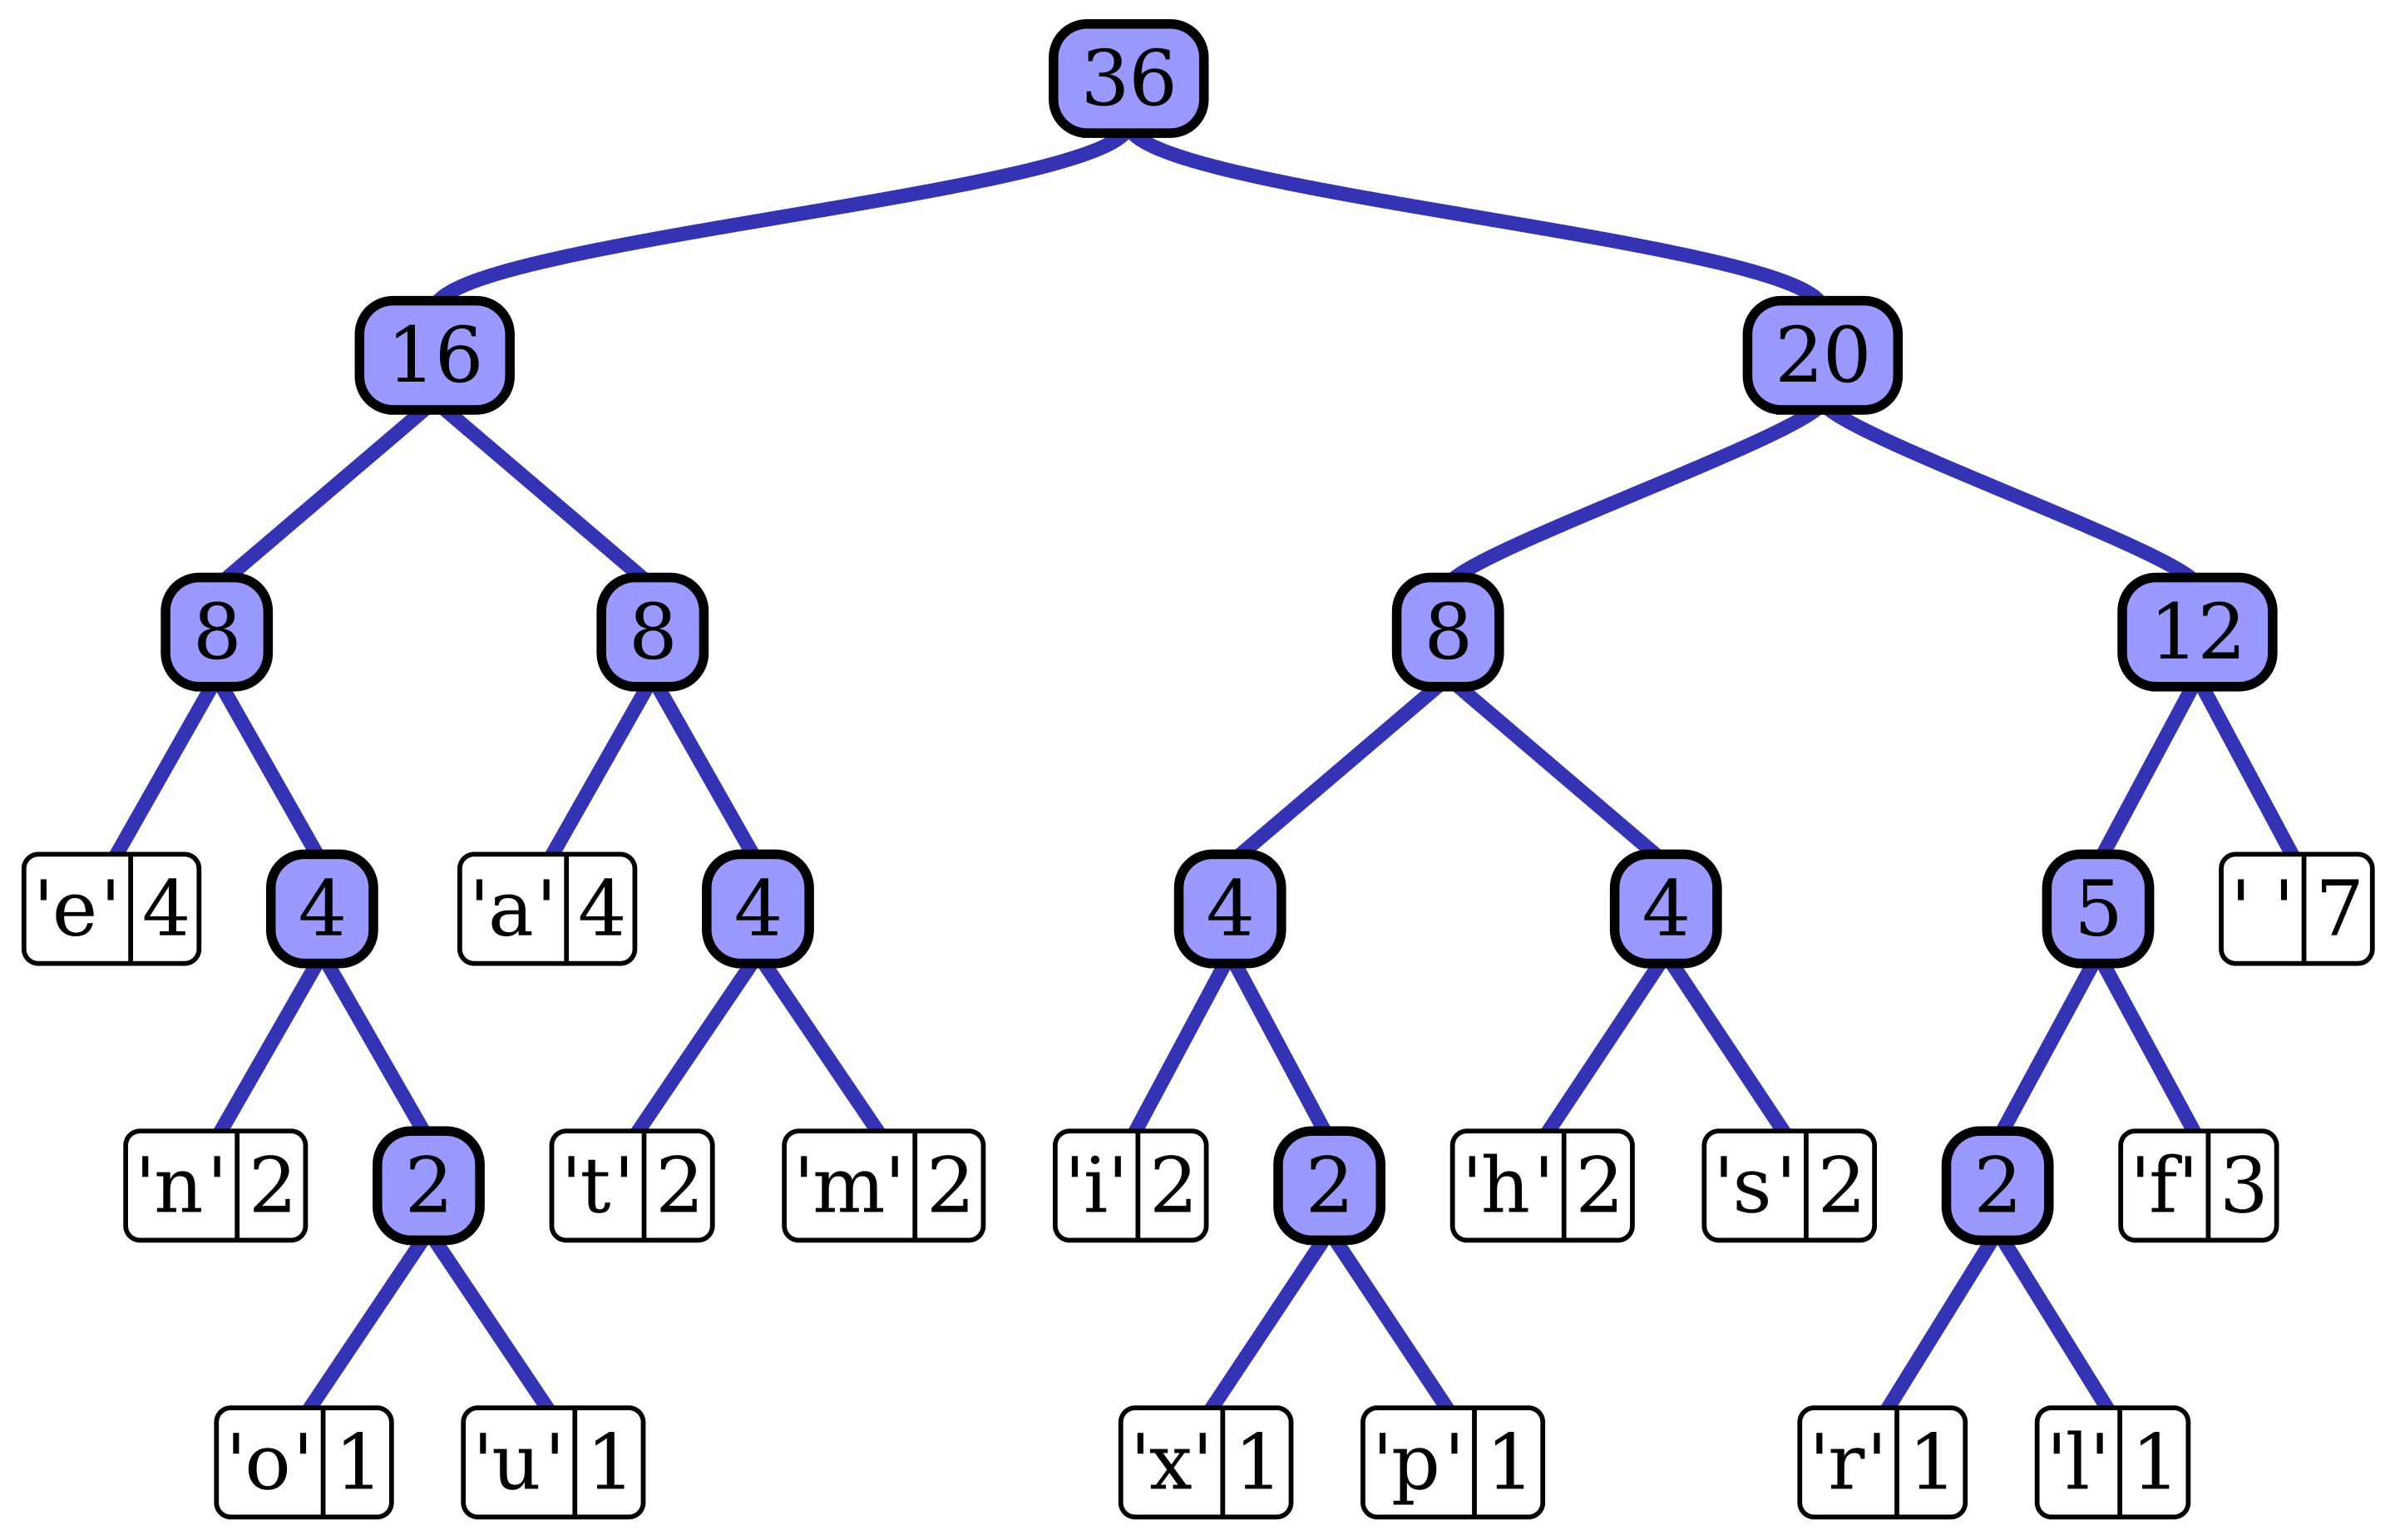
\includegraphics[scale=0.16]{img/huffmanTree.png}
    \caption{Huffman tree produced from "this is an example of a huffman tree"}
    \label{fig:my_label}
\end{figure}
So what's happening there ? Here we have a binary which have special leaves.\\
Those leaves contains two things, a character and a number, which corresponds to the number of occurences of its associated character.\\
\\
This tree was build using the frequency of each character, here is the algorithm used :
\begin{verbatim}
1. We take the two characters appearing the less.
2. We put them in leaves, which we'll make childs of a new node.
3. We compute in this new node the sum of the occurences of its two childs
4. Now we consider this new node has a possible child with the occurences computed previously
5. We repeat this process until there is no more leaves available
\end{verbatim}
But, what's the point of having this tree ? I'll show it to you with the following image :
\begin{figure}[H]
    \centering
    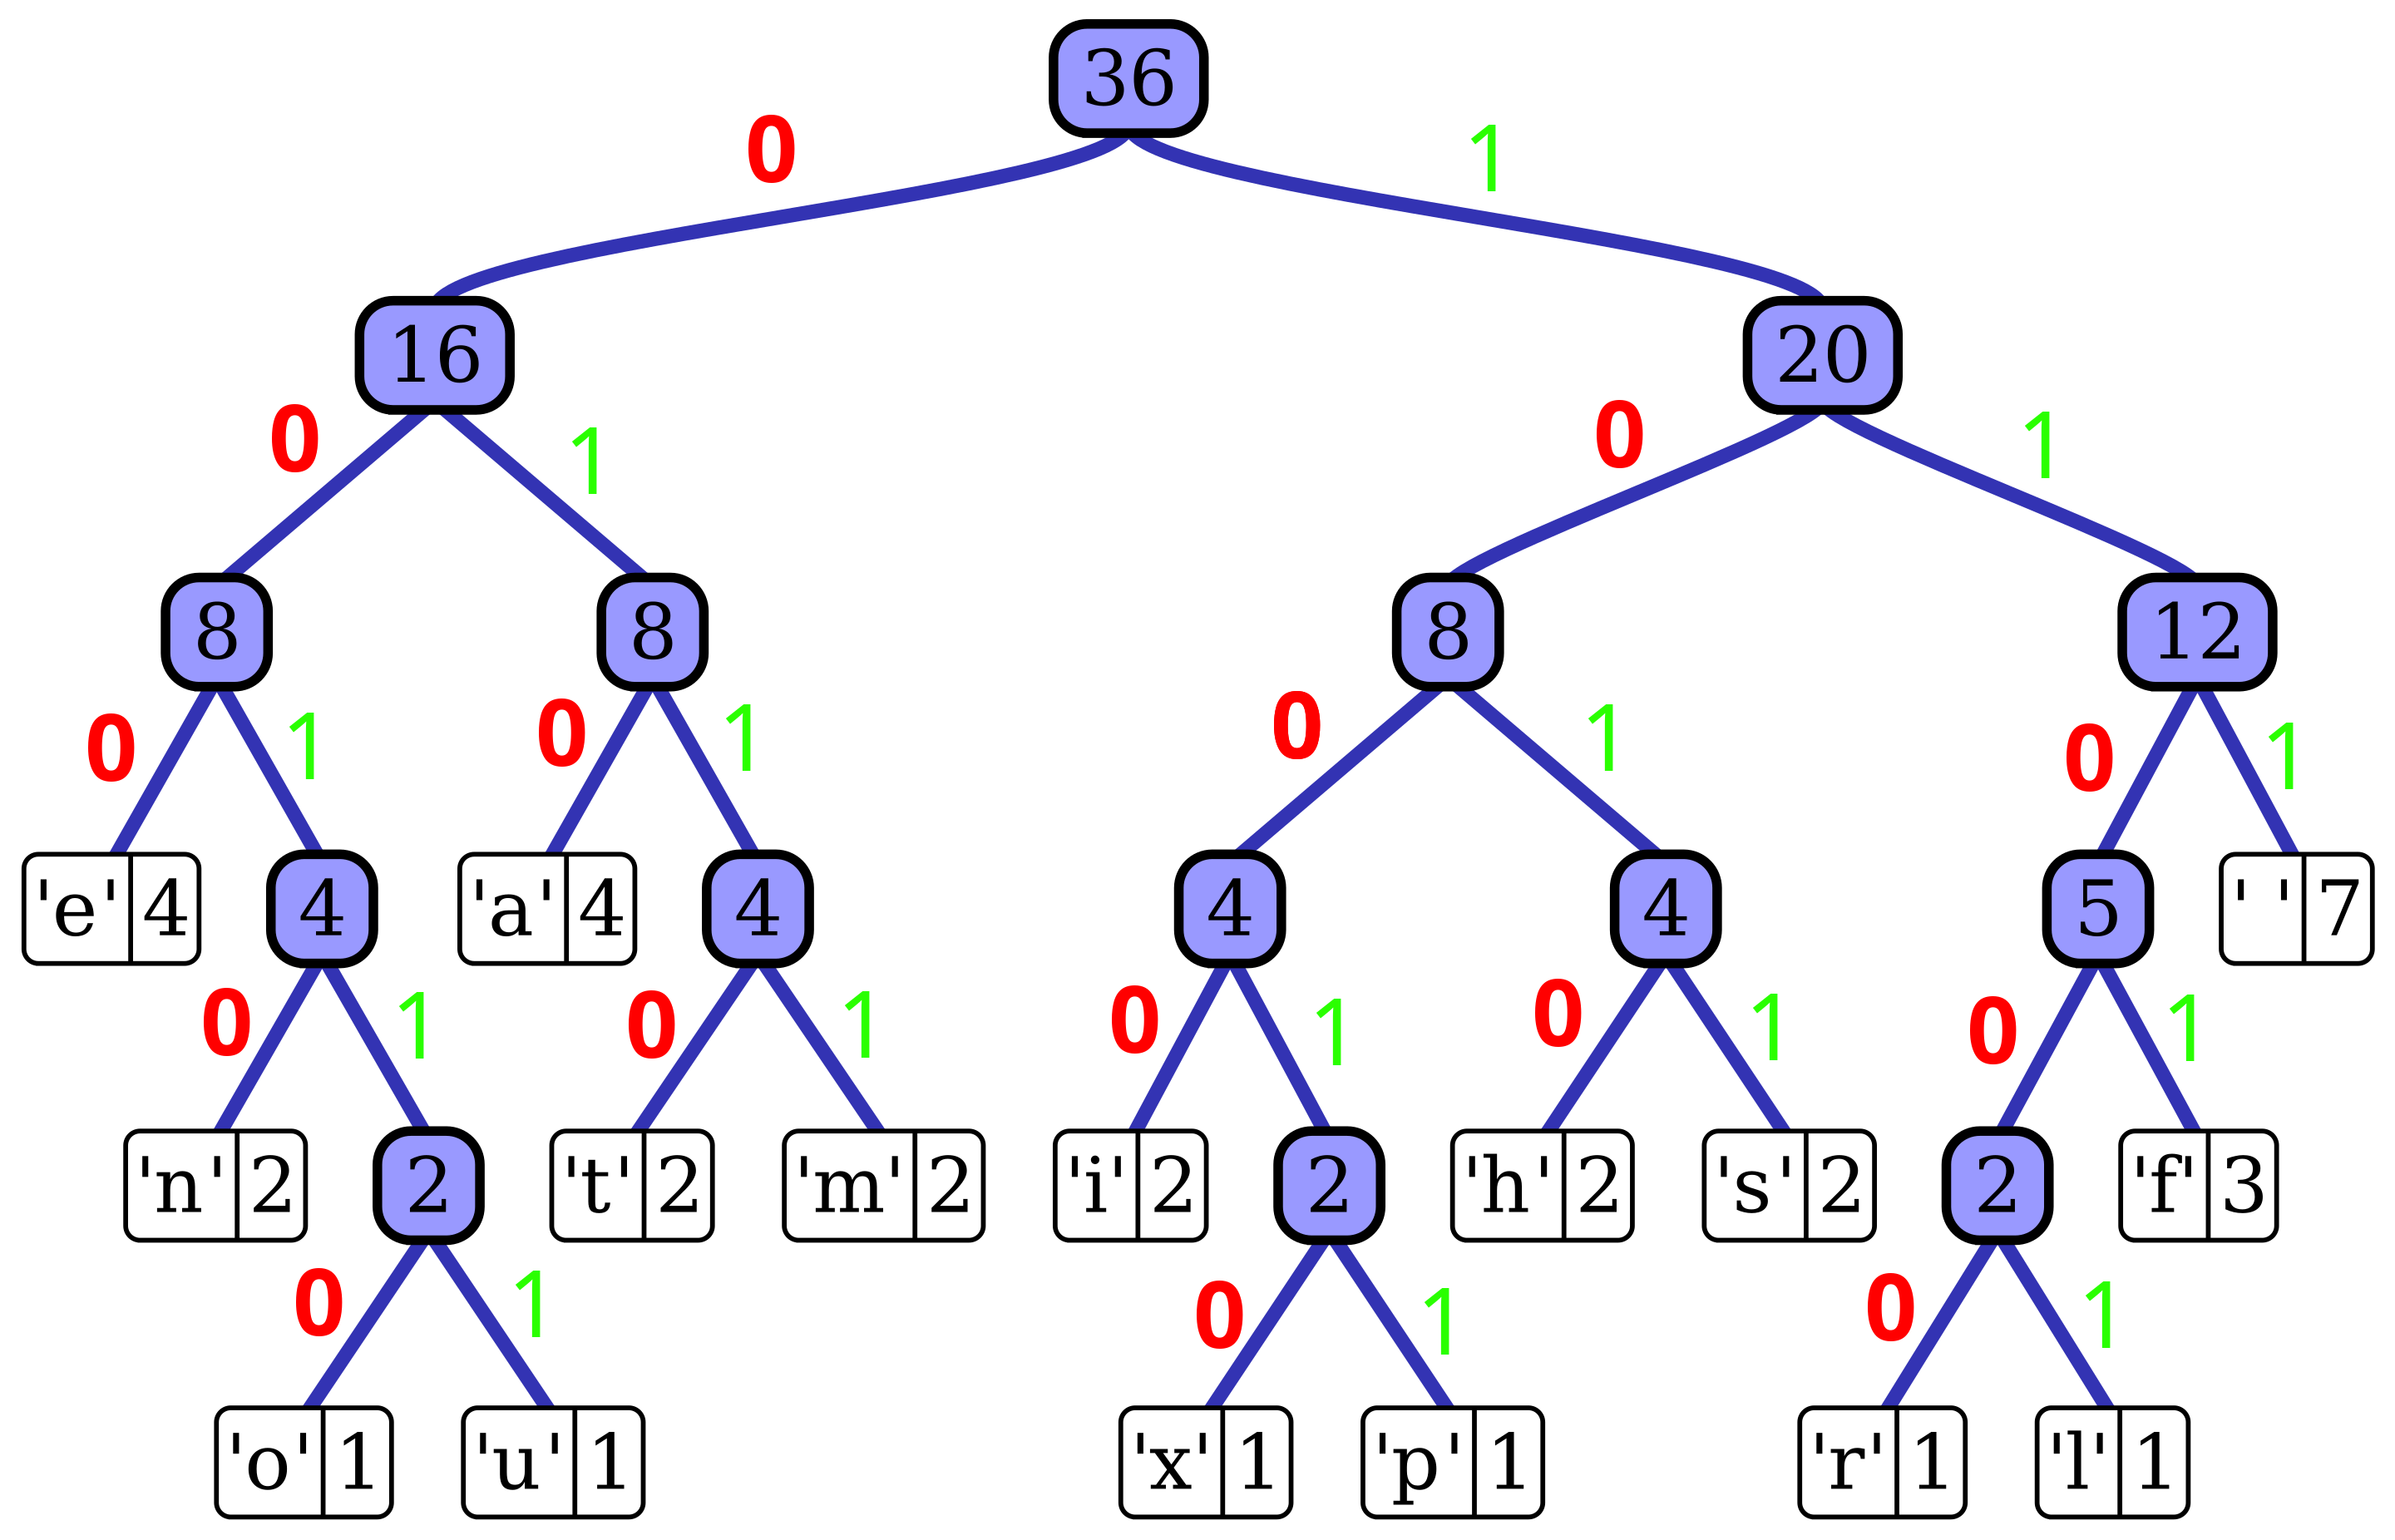
\includegraphics[scale=0.16]{img/huffmanTreeE.png}
    \caption{Huffman tree used for the encoding}
    \label{fig:my_label}
\end{figure}
The next step after building the tree is, generate the encoding.\\
This is done following a simple principle, the encoding of a character corresponds to its path in the tree. When we have to go through the left child of a node to go to the character leaf, we add a '0' to its encoding, and a '1' if we need to go through the right child.\\
For example, for the character 'p' we'll have : "10011".\\
Using this, it is quite easy to generate an encoding for each character, but it also very easy to decode a file.\\
\\
Let's imagine we're decompressing a file contaning these "10011 11000 000 000 1011" (the file will not actually containe these, it will contain the characters encoding by those bits).\\
In order to decode this, we'll simply have to explore the tree following the direction given by the bit.\\
For example, for "10011", we'll go right, left, left, right and finally right, and we would end up in the leaf of the character "p". After that we can go back to the root and begin to do that again.\\
\\
And this is where one property of this encoding is interesting, using this algorithm we generate what we call a "prefix encoding", which is an encoding where each code isn't suffix of any other. This property is fundamental for this algorithm.

\subsection{Padding issue}
Let's imagine we want to compress the following word "press", which is encoded by this "10011 11000 000 000 1011", here I have put spaces in order to make it more clear about which sequence corresponds to which character, but in reality this isn't that simple.\\
In our file, we're only writting characters, sequence of bytes, so our algorithm would rather write it this way "10011110 00000000 1011". And there is the issue, we can't write half a byte in a file, so our last sequence needs to be completed, to be larger.\\
We could simply add 4 zeros in order to have a full byte but we would still have an issue, if in our new encoding there is a character encoded by "0", "00", "000", or "0000", we would decode a character that wasn't in the original file.\\
\\
I found 2 ways to fix this issue :
\begin{itemize}
\item Write in the metadata, how much data there is to read.\\
Using this, we can tell the decompresser when to stop while reading the compressed data.\\
But, this would be an issue for our MPI version, well not quite an issue, but it would complexify a bit the MPI version.
\item Write in the metadata, how much data there in excess.\\
Using this, we can tell the decompresser that it only have to decode \textbf{n} bits in the last byte.
\end{itemize}